% part_C: 원문 13쪽 "V. AGENTIC SC" ~ 19쪽 V.C 직전 (V.A, V.B), 그림 7--11

\section{에이전트형 의미 통신}

인간의 지각 과정은 선택, 조직화, 해석의 세 단계로 이루어진다 [107].
지각 과정에서 주변 환경의 정보 가운데 일부가 선택적으로 인식되고, 구조화된 표현으로 조직되며, 해석된다.
SC의 발전은 이러한 순차적 인지 과정에 견줄 수 있다.
예를 들어, 선택 단계는 DeepJSCC 같은 직관 기반 의미 통신(intuition-driven SC) 모델이 과업과 관련된 특징을 선택적으로 전송하는 모습으로 나타난다.
그 뒤에 등장한 추론 기반 의미 통신(reasoning-driven SC) 시스템에는 맥락적 추론 모듈이 들어가므로, 이 시스템은 조직화 단계에 해당한다.
이 궤적을 따르면, 다음 진화 단계는 자연스럽게 해석 단계를 겨냥해야 한다.
해석 단계에서는 맥락에 대한 이해와 적응적 추론을 통해 의미가 동적으로 구성된다.
통신 시스템에서 이 해석 단계를 구현하려면, 에이전트는 맥락에서 의미를 추론할 뿐 아니라 통신 제약 아래에서 그 의미에 따라 어떻게 행동할지도 결정해야 한다.

\setcounter{figure}{6}
\begin{figure}[htbp]
\centering
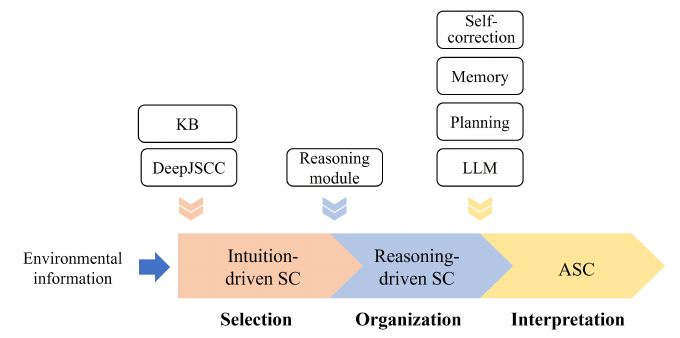
\includegraphics[width=\linewidth]{fig/fig7.png}
\caption{인간의 지각 과정과 의미 통신의 진화 궤적 사이의 개념적 대응.}
\label{fig:7}
\end{figure}

이러한 맥락에서 ASC의 에이전트적 성격은, 정적인 프로토콜에서 벗어나 의미를 추론할 뿐 아니라 협상하기도 하는 동적 상호작용 과정으로 옮겨 가는 것이라고 정의할 수 있다 [108].
LLM은 이러한 창발적 행동을 계산적으로 실현할 수 있게 해 주는 핵심 기술 기반 가운데 하나다.
또한 LLM은 의미 추상화 [109], 맥락적 추론 [110], 처음 보는 입력에 대한 맥락 내 일반화 [110] 능력을 바탕으로 자율적 상호작용을 뒷받침한다.
계획, 메모리, 자기 교정 모듈의 지원을 받으면 LLM은 표현을 발전시키고, 행동의 결과를 예측하며, 전략을 지속적으로 개선할 수 있다.
이러한 메커니즘을 통해 ASC는 에이전트들 사이의 자율적 교환에서 의미가 창발하는 해석 단계를 구현한다.
지각 과정과 의미 통신의 기능 사이의 관계를 그림~7에 나타냈다.

\subsection{ASC의 핵심 구성 요소}

\paragraph{1) 에이전트}
ASC에서 에이전트는 내부 상태와 맥락적 이해를 바탕으로 의미 표현을 생성하고, 해석하고, 발전시키는 데 참여하는 의미적 개체로 본다.
기존 시스템에서 송신기와 수신기는 수동적인 의미 압축기와 압축 해제기로 간주된다.
이와 달리 ASC의 에이전트는 직관과 추론을 모두 아우르는 인지 능력을 갖춘 능동적 참여자로 가정한다.

\paragraph{2) 지각}
ASC 루프는 지각(perception)으로 시작될 수 있다.
지각은 환경 상태를 국소 관측으로 사상하고, 의미 부호기는 이 국소 관측에서 의미 잠재 상태를 추출한다(V-A6절에서 정식화한다).
지각된 의미 잠재 상태는 과업 의도, 메모리, KB 상태, 채널 정보와 함께 무엇을 전송할지에 관한 결정, 전송할 의미, 세계 모델 예측에 의존할지 여부에 영향을 주는 조건이 된다.
따라서 지각은 암묵적 입력이 아니라 명시적인 기능 모듈로 다룰 수 있다.

\paragraph{3) 지식 베이스}
ASC에서 KB는 온톨로지, 제약, 사실, 규칙을 담은 공유 저장소 역할을 하며, 송신기와 수신기가 이를 동적으로 동기화한다고 가정한다 [111].
송신기는 KB를 사용해 원시 데이터를 의미 표현으로 부호화한다 [20].
복호기는 KB를 활용해 낮은 신호 대 잡음비(SNR) 조건에서도 데이터를 강인하게 복원한다.
ASC 프레임워크는 맥락 정보를 부호화하는 데 그치지 않고, KB의 지속적인 갱신과 정렬을 통해 공유되고 구조화된 언어가 동적으로 공진화한다고 가정한다.
상호작용을 통한 이러한 프로토콜 적응은 V-C절에서 논의한다.

\paragraph{4) 세계 모델}
세계 모델은 일종의 꿈 엔진(dream engine)으로 기능한다.
세계 모델 덕분에 에이전트는 미래의 의미 잠재 상태, 곧 미래 환경 상태를 과업에 맞게 추상화한 것을 예측하고, 가능한 행동의 결과를 평가하며, 과업을 실행하기 전에 의사 결정을 뒷받침할 수 있다.
이에 따라 세계 모델은 에이전트가 환경 안에서 자기 행동의 결과를 예측할 수 있게 해 준다 [112].
체화 AI(embodied AI)와 로봇공학 분야에서는 세계 모델이 일관된 미래 예측을 바탕으로 감각운동 제어와 추론을 연결하여, 분포 밖(OOD) 상황에 대한 강인성을 높일 수 있음이 입증되었다 [113].
Ha와 Schmidhuber [112]는 세계 모델 기반 파이프라인을 제시하고, 구성된 ``꿈'' 환경에서 학습한 정책을 실제 환경으로 옮길 수 있음을 보였다.
컴퓨터 비전 분야에서는 비디오 시퀀스를 예측하여 물리적 동역학을 포착하는 WorldDreamer [114]가 제안되었다.

ASC 안에서 세계 모델은 송신기 쪽에서 \textit{의미 상태 기술자(semantic state descriptor)} 역할을 할 수 있다.
이 구성 요소는 숨은 동역학을 추론하여 의미 정보를 효율적으로 부호화할 수 있게 한다.
수신기 쪽에서는 세계 모델을 \textit{청자 의미 추론(listener semantic inference)}으로 구현한다.
이 구성 요소는 복원된 의미 잠재 상태 위에서 이루어지는 후속 기호 추론을 뒷받침하여 과업을 더 효과적으로 수행한다.
이러한 메커니즘을 통해 세계 모델은 에이전트가 이미 확립된 개념을 활용해 처음 보는 시나리오에서도 합리적인 결정을 내리게 해 준다.

세계 모델은 전송 효율과 추론 측면에서 ASC 프레임워크를 강화할 수 있다.
세계 모델은 과업 보상에 따라 중간 추론 상태를 생성하여 행동 공간의 불필요한 탐색을 줄이는 데 쓰였다 [115].
또한 압축에 쓰일 때 세계 모델은 원시 관측 대신 궤적을 예측하여 전송 정보량을 줄인다 [116].
더 나아가, 환경의 구조적 의존성을 학습함으로써 세계 모델을 갖춘 프레임워크는 분포 이동 아래에서도 안정적인 성능을 유지할 수 있다 [43].
이러한 활용은 V-B1절에서 논의한다.

\paragraph{5) 의미 메모리}
맥락 정보를 보강하는 KB와 달리, 의미 메모리(semantic memory)는 전송된 의미 표현(SR, semantic representation)을 저장하고 검색한다.
통신 세션 동안 의미 메모리는 SR을 보관해 뒤이은 패킷 전송에서 다시 사용하며, 이로써 대화의 연속성을 높인다 [117].
의미 메모리는 세션마다 다르며 온라인으로 갱신된다.
맥락 보강과 데이터량 감축을 위한 대표적인 활용 사례는 V-B3절에서 살펴본다.

\paragraph{6) ASC의 수학적 추상화}
여기서는 ASC의 통신 과정과 추론 과정을 수학적으로 추상화하여 기술한다.
정식화에는 관측, 의미 잠재 상태, KB, 세계 모델, EmLang 토큰, 채널 상태, 과업 효용이 포함된다.
이 요소들을 바탕으로 ASC 에이전트는 \textit{어떤} 의미 정보를 전송할지, \textit{언제} 전송할지, 수신한 정보를 추론이나 추리에 \textit{어떻게} 사용할지를 결정한다.
먼저 ASC 에이전트의 기능적 구조를 정의한 뒤, 세계 모델 기반 송수신기 상호작용을 예로 들어 기술한다.
이 추상화의 목적은 유일한 시스템 모델을 규정하는 것이 아니라, ASC의 통신과 추론의 바탕에 있는 기능적 역할과 가정을 밝히는 데 있다.

인터페이스 공간, 내부 상태 공간, 기능 모듈, 결정 계층을 구분하기 위해 ASC 에이전트 $i$를 다음과 같이 나타낸다.
\begin{equation}
\mathcal{A}_i = (\mathcal{I}_i,\, \mathcal{Z}_i,\, \mathcal{M}_i,\, \mathcal{D}_i), \tag{1}
\end{equation}
여기서 $\mathcal{I}_i = (\mathcal{O}_i, \mathcal{U}_i, \mathcal{L}_i, \mathcal{C}_i, \mathcal{R}_i)$는 인터페이스 공간을 모은 것으로, 국소 관측 공간 $\mathcal{O}_i$, 국소 행동 공간 $\mathcal{U}_i$, 의미 토큰 공간 $\mathcal{L}_i$, 채널 상태 공간 $\mathcal{C}_i$, 통신 자원 행동 공간 $\mathcal{R}_i$로 이루어진다.
$\mathcal{Z}_i = (\mathcal{S}_i, \mathcal{H}_i, \mathcal{K}_i)$는 내부 상태 공간을 모은 것으로, 의미 잠재 공간 $\mathcal{S}_i$, 내부 상태 공간 $\mathcal{H}_i$, 국소 KB 상태 공간 $\mathcal{K}_i$로 이루어진다.
$\mathcal{M}_i = (P_i, E_i, \mathcal{W}_i)$는 기능 모듈을 모은 것으로, 지각 함수 $P_i$, 의미 부호기 $E_i$, 그리고 (2)의 세계 모델 모듈 $\mathcal{W}_i$로 이루어진다.
$\mathcal{D}_i = (\pi_i, J_i)$는 결정 계층으로, (3)의 결합 행동-통신 정책 $\pi_i$와 $\pi_i$가 최대화하는 과업 수준 효용 $J_i$로 이루어진다.
이 묶음들은 필수 구성 요소가 아니라 분석상의 역할로 해석해야 한다.
예를 들어 예측 모델링을 쓰지 않는 ASC 구현은 $\mathcal{W}_i$를 생략하거나 다른 것으로 바꿀 수 있다.

\textit{상태 표기.}
환경 상태는 물리적 환경의 실제 상태로 정의한다.
지각 함수 $P_i$는 이 상태를 국소 관측 $o_i^t$로 사상하고, 의미 부호기 $E_i$는 이 관측에서 의미 잠재 상태 $s_i^t = E_i(o_i^t, k_i^t)$를 추출한다.
의미 잠재 상태는 과업과 관련된 간결한 표현이다.
내부 상태는 의미 메모리와 관측 이력을 요약한다.
KB 상태 $k_i^t$와 $k_j^t$는 국소 지식 상태를 나타내며, 특정 구현이 공유 KB에 의존할 때 동기화된다.
채널 상태는 링크 조건을 기술한다.
신념 상태(belief state)는 다중 에이전트 조정을 고려할 때만 도입한다.
따로 밝히지 않는 한, 이 정식화의 나머지 부분에서 ``상태''는 의미 잠재 상태를 가리킨다.

통신과 추론을 결합하는 데 예측을 사용하는 ASC 구현을 생각하자.
에이전트 $i$는 다음 의미 잠재 상태를 다음과 같이 예측한다.
\begin{equation}
\hat{s}_{i,t+1} = \mathcal{W}_i(s_{i,t},\, u_i^t;\, k_i^t), \tag{2}
\end{equation}
여기서 $t$는 이산 시간 슬롯 인덱스, $s_{i,t}$는 현재 의미 잠재 상태, $u_i^t$는 제어 행동, $k_i^t$는 국소 KB 상태다.
예측한 다음 상태 $\hat{s}_{i,t+1}$은 추론을 위한 의미적 사전 정보(semantic prior)로 쓰인다.

송신기 $i$에서 수신기 $j$로 가는 통신 링크에서, 송신기는 내부 상태 $h_i^t$, KB 상태 $k_i^t$, 채널 상태 $c_{ij}^t \in \mathcal{C}_i$를 고려하여 무엇을 전송하고 자원을 어떻게 할당할지 선택한다.
전송 시점은 아래에서 따로 구체화한다.
구체적으로, 송신기는 결합 정책을 통해 제어 행동 $u_i^t$, EmLang 토큰 시퀀스 $\ell_{i\to j}^t \in \mathcal{L}_i$, 자원 벡터 $\rho_{ij}^t \in \mathcal{R}_i$를 다음과 같이 선택할 수 있다.
\begin{equation}
(u_i^t,\, \ell_{i\to j}^t,\, \rho_{ij}^t) \sim \pi_i(\cdot \mid h_i^t, k_i^t, c_{ij}^t). \tag{3}
\end{equation}
전송 결정 $a_{ij}^t \in \{0,1\}$은 (3)의 정책이 출력하는 값이 아니다.
이 값은 아래 (4)의 결정론적 사건 트리거로 정해진다.
이 트리거는 \textit{언제} 전송할지를 정하는 한 가지 구현일 뿐이며, 다른 ASC 설계에서 학습 기반 또는 규칙 기반 전송 결정을 쓰는 것을 배제하지 않는다.
또한 자원 벡터 $\rho_{ij}^t$는 자원 요청(예: 원하는 전송률과 의미적 우선순위)으로 해석하며, 하위의 매체 접근 제어(MAC) 스케줄러가 이를 물리 무선 자원에 사상한다.

세계 모델 기반의 경우에서 \textit{언제} 전송할지의 결정을 명시적으로 만들기 위해, 예측한 의미 잠재 상태와 관측한 의미 잠재 상태 사이의 불일치로 통신을 트리거할 수 있다.
슬롯 $t$ 안에서 제어 행동 $u_i^t$를 먼저 적용하고, 그다음 새 관측에서 의미 잠재 상태 $s_{i,t+1}$을 추출한다.
다음과 같이 정의한다.
\begin{equation}
\epsilon_{i,t} = d_s(s_{i,t+1}, \hat{s}_{i,t+1}), \qquad
a_{ij}^t =
\begin{cases}
1, & \epsilon_{i,t} \ge \epsilon_{\mathrm{th}},\\
0, & \text{그 외},
\end{cases} \tag{4}
\end{equation}
여기서 $\epsilon_{\mathrm{th}}$는 건너뛰기 임곗값이고, $d_s(\cdot,\cdot)$는 의미 잠재 공간에서 정의한 과업 의존 불일치 척도다.
잠재 표현이 유클리드 기하를 허용하면 유클리드 거리를 한 가지 선택으로 쓸 수 있다.
여기서 $a_{ij}^t = 1$은 에이전트 $i$에서 에이전트 $j$로 의미를 전송함을 나타내고, $a_{ij}^t = 0$은 의미를 전송하지 않음을 나타낸다.
(4)의 사건 트리거는 이 구현의 전송 시점 규칙이다.
(1)의 에이전트 수준 표현을 바꾸지 않고도 학습된 트리거나 과업 특화 트리거로 이를 대체할 수 있다.

전송하지 않는 경우, 예측 오차는 환경을 관측하는 유일한 쪽인 송신기에서 측정한다.
표기를 간단히 하기 위해, 활성 링크 하나만 고려할 때는 $\epsilon_t$를 쓴다.
$a_{ij}^t = 1$이면 토큰 시퀀스 $\ell_{i\to j}^t$는 실제 의미 잠재 상태 $s_{i,t+1}$ 또는 $\hat{s}_{i,t+1}$에 대한 그 잔차를 나타내며, 송신기는 예측 상태와 KB를 맥락 정보로 삼아 토큰을 채널 심볼로 부호화한다.
$a_{ij}^t = 0$이면 의미 페이로드를 전송하지 않는다.

수신기에서는 $a_{ij}^t = 1$일 때 성공적으로 복호한 토큰으로 사후 잠재 상태를 $\tilde{s}_{j,t+1} = \phi_j(\hat{\ell}_{i\to j}^t, k_j^t)$로 갱신한다.
그렇지 않으면 수신기는 자신의 국소 예측, 곧 $\tilde{s}_{j,t+1} = \hat{s}_{j,t+1}$을 사용한다.
$a_{ij}^t = 1$일 때의 채널 신뢰도를 $q_{ij}^t \in [0,1]$이라 하고, $a_{ij}^t = 0$일 때는 $q_{ij}^t = 1$로 둔다.
전송하지 않는 경우에 $q_{ij}^t = 1$로 두는 것은, 의도적인 건너뛰기를 수신기가 식별할 수 있다고 가정하는 것이다.
예를 들어 가벼운 1비트 건너뛰기 표시나 미리 합의한 전송 일정을 통해 식별하면, 건너뛰기를 패킷 손실과 혼동하지 않는다.

수신기는 전환 함수를 통해 의미 상태 불일치와 채널 불확실성을 결합할 수 있다.
\begin{equation}
\xi_{ij,t} = \Gamma\bigl(\epsilon_{ij,t},\, 1 - q_{ij}^t\bigr), \tag{5}
\end{equation}
여기서 $\epsilon_{ij,t} = d_s(\tilde{s}_{j,t+1}, \hat{s}_{j,t+1})$는 $a_{ij}^t = 1$일 때 사후 잠재 상태와 국소적으로 예측한 잠재 상태 사이의 불일치를 나타낸다.
함수 $\Gamma(\cdot,\cdot)$는 예측 불일치와 채널 불확실성을 추론 전환 점수로 사상한다.
간단한 가중합 구현은 $\Gamma(\epsilon, 1-q) = \epsilon + \lambda(1-q)$이며, $\lambda \ge 0$이 채널 불확실성의 영향을 조절한다.

$a_{ij}^t = 0$이면 수신기는 이 오차를 국소적으로 측정할 수 없으므로, 보수적인 대리값 $\epsilon_{ij,t} = \epsilon_{\mathrm{th}}$로 대신한다.
이 값은 (4)에서 송신기가 측정한 오차의 상한이다.
이 근사는 송신기와 수신기의 세계 모델이 동기화되어 있다고 가정한다.
이에 따라 전환 임곗값은 $\Gamma(\epsilon_{\mathrm{th}}, 0) < \xi_{\mathrm{th}}$가 되도록 정한다.
그러면 채택한 대리값 아래에서 의도적인 건너뛰기는 시스템 1(System 1) 경로를 따른다.
수신기 출력은 다음과 같다.
\begin{equation}
\hat{x}_j^t =
\begin{cases}
f_{\mathrm{S1}}(\tilde{s}_{j,t+1},\, k_j^t), & \xi_{ij,t} < \xi_{\mathrm{th}},\\
f_{\mathrm{S2}}(\tilde{s}_{j,t+1},\, k_j^t,\, \hat{s}_{j,t+1}), & \xi_{ij,t} \ge \xi_{\mathrm{th}},
\end{cases} \tag{6}
\end{equation}
여기서 $f_{\mathrm{S1}}$은 빠른 추론 경로, $f_{\mathrm{S2}}$는 추리 경로를 나타낸다.
따라서 시스템 1/시스템 2 전환은 세계 모델 불일치와 채널 불확실성을 모두 반영한다.

\textit{세계 모델 동기화.}
건너뛰기 메커니즘이 작동하려면 송신기와 수신기가 공유된 잠재 기준 상태(latent anchor state)에서 출발해 진화하는 동기화된 세계 모델을 실행해야 한다.
이 동기화를 유지하기 위해 두 종류의 정보를 교환한다.
첫째는 모델 파라미터 갱신으로, 예정된 갱신 단계(예: $T_{\mathrm{model}}$ 슬롯마다)에 낮은 빈도로 동기화하거나, 누적된 파라미터 차이가 허용치를 넘을 때 사건 트리거 방식으로 동기화한다.
갱신 주기는 응용의 시간 척도에 맞추어 정한다.
반면 잠재 기준 상태는 실제 전송이 일어날 때마다 갱신된다.
기준 상태를 갱신할 때마다 관련 제어 행동 $u_i^t$도 함께 전달되므로, 수신기는 건너뛰는 슬롯 동안 송신기와 함께 조건부 세계 모델을 실행할 수 있다.
이때 건너뛰는 동안의 의미 표류(semantic drift)는 하트비트 규칙으로 제한할 수 있다.
예를 들어 최대 $N_{\max}$개의 연속 슬롯을 건너뛴 뒤에는 송신기가 $\epsilon_{i,t}$와 상관없이 현재 의미 잠재 상태를 전송한다.
이러한 동기화 조건은 예측 기반 건너뛰기에서 생기는 것이며, 동기화된 수신기 측 예측기에 의존하지 않는 구현에는 필요하지 않다.

\textit{의도 정렬.}
$g_i^t = \psi_i(h_i^t)$와 $\hat{g}_{j\leftarrow i}^t = \varphi_j(\tilde{s}_{j,t+1},\, h_j^t)$가 각각 송신기 $i$의 과업 의도와 수신기 $j$가 추론한 의도를 나타낸다고 하자.
여기서 $\psi_i(\cdot)$와 $\varphi_j(\cdot)$는 과업 의존 사상이다.
의도 수준의 의미 정렬은 $A_{ij}^t = \mathrm{sim}(g_i^t, \hat{g}_{j\leftarrow i}^t)$로 정량화할 수 있고, 그 시간 평균 $\frac{1}{T}\sum_{t=1}^{T} A_{ij}^t$는 한 에피소드에 걸친 의도 보존 정도를 평가한다.

\textit{조정 메커니즘.}
다중 에이전트 ASC 시스템에서 각 에이전트 $i$는 과업과 관련된 신념 상태 $b_i^t = B_i\bigl(h_i^t,\, \{\hat{\ell}_{j\to i}^t\}_{j\in\mathcal{N}_i}\bigr)$를 유지한다.
전송 결정을 바탕으로 활성 통신 링크의 집합을 $E_t = \{(i,j) : a_{ij}^t = 1\}$로 정의한다.
그러면 보편적으로 규정된 조정 목표 대신 $\max_{(i,j)\in E_t} d(b_i^t, b_j^t)$와 같은 과업 의존 발산 기준을 통해 의미적 일관성을 유도할 수 있다.

\textit{범위와 한계.}
이 수학적 추상화는 이 서베이에서 다루는 ASC 구성 요소를 정리하고, 이를 통신, 예측, 추론, 결정 과정과 연결하기 위한 공통 표기를 제공한다.
기존 연구는 프레임워크의 서로 다른 부분에 대응시킬 수 있다.
예측적 계획은 세계 모델과 건너뛰기 규칙 (4)에 대응하고(V-B1절), EmLang 기반 방법은 토큰 공간에 대응하며(V-C절), 메모리 기반 방법과 검색 증강 생성(RAG) 기반 방법은 내부 상태와 KB 상태에 대응하고(V-B3절), 다중 에이전트 강화학습(MARL) 기반 접근은 정책에 대응한다(V-E절).
ASC 시스템에 따라 세계 모델, 결정론적 건너뛰기, 공유 KB, 시스템 1/시스템 2 전환이 필요하지 않을 수도 있다.
학습 절차, 동기화 오버헤드, 종단 간 시스템 검증은 이 서베이의 범위를 벗어난다.

\subsection{ASC의 에이전트 수준 자율성}

LLM은 추론 기반 의미 통신 시스템에서 유망한 모델로 활용되어 왔지만 [44], [76], [118], 적응성이 제한적이어서 자율성에 제약이 있다.
또한 LLM을 사용한 상호작용은 시스템에 추가 부담을 준다.
토큰 처리 때문에 에이전트가 한 번의 추론 주기 안에서 활용할 수 있는 시간적·다중 모달 맥락이 제한된다.
따라서 LLM으로 자율성을 구현하려면 계산 효율적인 설계와 함께 동적 계획, 메모리, 자기 교정 능력이 필요하다.
이 구성 요소 전반에 걸쳐 DRL은 ASC 시스템의 자율 적응을 위한 핵심 메커니즘을 제공할 수 있다.
구체적으로, DRL은 세계 모델을 이용한 예측적 계획 [115], 자기 교정 모듈을 이용한 자율적 오류 교정 [119], 다중 에이전트 환경에서의 협력적 정책 최적화 [120]를 돕는다.

\paragraph{1) 세계 모델을 이용한 예측적 계획}
세계 모델은 ASC를 기존 의미 통신 개념과 구별해 주는 핵심 구성 요소 가운데 하나다.
LLM은 과업 특화 학습에는 능숙하지만 복잡한 동역학을 포착하는 데에는 자주 어려움을 겪는다 [115].
세계 모델은 에이전트가 주어진 맥락에서 결과를 시뮬레이션하고 예측할 수 있게 해 주는 내부 인지 모듈로 기능한다.

LLM의 추론 능력과 세계 모델의 예측 능력을 결합함으로써 ASC는 엣지 일반 지능(EGI, edge general intelligence)과 유사한 프레임워크를 구축한다 [121].
그림~8([121]에서 착안)에 보인 것처럼, 세계 모델 기반 ASC 프레임워크는 시뮬레이션과 실행의 역할을 분리한다.
LLM 기반 에이전트로 구성된 \textit{상호작용 프런트엔드(Interaction Frontend)}는 실세계의 지각과 실행을 담당한다.
반면 세계 모델이 구동하는 \textit{인지 백본(Cognitive Backbone)}은 관측을 부호화하여 예측된 의미 잠재 상태를 도출한다.
상태 예측 구성 요소는 (2)에 해당하며, 기대 보상은 예측된 상태 위에서 보조 보상 평가기가 추정한다.
이 보상은 과업 성능을 최대화하는 행동을 선택하기 위한 지침으로 쓰인다.
지각--예측--행동 루프를 통해 에이전트는 전송 전략을 적응적으로 결정한다.
전체 과정은 다음과 같다.
환경 인식, 의미 잠재 상태 추출, 세계 모델 예측, 전송 결정(건너뛰기 또는 전송), LLM 계획과 자원 할당, 공유 KB를 이용한 의미 토큰 생성, 수신기 추론, 그리고 모델이나 KB에 대한 되먹임 기반 갱신을 통한 세계 모델 재동기화다.
이 나열은 한 슬롯 안의 엄밀한 시간 순서가 아니라 한 번의 닫힌 주기에서의 정보 흐름을 기술한다.
(2)의 세계 모델 예측은 계획기(planner)가 선택한 제어 행동을 조건으로 하며, (4)의 전송 결정은 행동이 실행되고 새 의미 잠재 상태가 추출된 뒤에 내려진다.

\setcounter{figure}{7}
\begin{figure}[htbp]
\centering
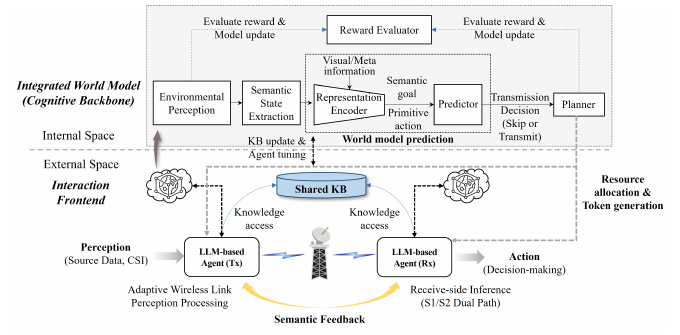
\includegraphics[width=\linewidth]{fig/fig8.png}
\caption{세계 모델 기반 ASC의 폐루프 작업 흐름.}
\label{fig:8}
\end{figure}

세계 모델은 ASC 안에서 두 가지 기능 모듈로 쓰였다.
하나는 통신 인지 동역학 모듈 [115], [122], [123]이고, 다른 하나는 추상화 모듈 [124], [125]이다.
통신 인지 동역학 모듈로 쓰일 때 세계 모델은 미래 행동과 맥락을 고려하여 각 잠재 상태의 효용을 예측한다.
추상화 모듈은 다중 모달 입력을 의미 잠재 상태로 부호화한다.

통신 인지 모듈의 사례로, 최근 연구 [122]는 몬테카를로 트리 탐색을 통합하여 LLM을 세계 모델로 사용한다.
이 프레임워크에서 LLM은 과업 보상의 안내를 받는 추론 트리를 점진적으로 구성한다.
이 방법은 추론 과업에서 사고 사슬(CoT, chain-of-thought) [35] 기준선보다 우수한 성능을 보였다.
또한 LLM은 규칙 학습을 통해 세계 모델로 기능할 수 있다 [123].
에이전트의 궤적을 세계 모델의 예측과 비교함으로써, 이 접근은 기존 에이전트보다 높은 성공률, 빠른 재계획, 낮은 토큰 비용을 달성한다.
이 결과는 LLM 기반 세계 모델이 과업 수준 계획에 효과적일 수 있음을 시사한다.
다만 계산 비용 때문에 시간 제약이 매우 엄격한 통신 루프에서는 여전히 사용이 제한될 수 있다.
이 결과는 [122], [123]에서 일반 추론 벤치마크에 대해 보고된 것이며, 지연 제약이 있는 통신 루프에 적용할 수 있는지는 아직 검증되지 않았다.

세계 모델은 에이전트가 압축된 의미 표현을 전송하게 하여 효율적인 전송을 뒷받침하는 데 쓰일 수 있다.
에이전트는 고차원 정보를 통째로 전송하는 대신, 내부 세계 모델을 사용해 정보를 부호화할 수 있다 [124], [125].
동기화된 세계 모델로 미래 의미 잠재 상태를 예측하고 예측 오차가 임곗값을 넘을 때만 실제 전송을 트리거하면, 전송을 아예 생략할 수도 있다 [116].
이로써 통신 오버헤드, 에너지 소비, 지연이 줄어든다 [116], [124].
더 나아가 세계 모델은 직관적 예측과 논리적 추론을 결합하여 계획을 보완하는 데 쓰일 수 있다 [125].
구현 단계에서 동역학 모듈은 학습된 전이 함수를 사용해 전송 전에 계획을 세운다.
추상화 모듈은 입력을 간결한 잠재 상태로 압축하여 과업이 독립적으로 실행될 수 있게 한다.
수신기의 세계 모델이 충분한 의미 충실도를 갖추면 전송을 건너뛸 수 있다.
이 과정은 V-E절에서 자세히 기술한다.

\setcounter{figure}{8}
\begin{figure}[htbp]
\centering
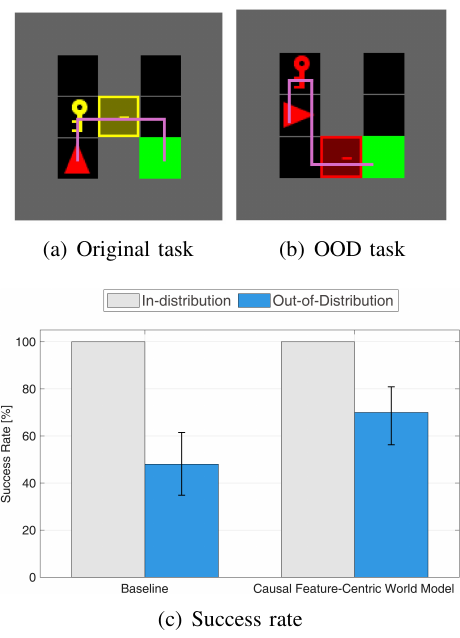
\includegraphics[width=0.6\linewidth]{fig/fig9.png}
\caption{인과적 특징 중심 세계 모델의 OOD 강인성에 대한 시뮬레이션 결과.}
\label{fig:9}
\end{figure}

또한 세계 모델은 OOD 조건에서 성능을 높일 잠재력이 있다.
[43]에서는 세계 모델이 인과적 특징에 집중함으로써 OOD 조건에서 일반화 성능을 높일 수 있음을 증명했다.
다른 연구 [126]은 텍스트 설명을 보조 입력으로 삼아 가려진 영역을 복원하도록 세계 모델을 학습시키면, OOD 조건에서 시각적 변화에 대한 강인성이 향상됨을 보였다.
우리는 OOD 강인성을 평가하기 위해 간단한 시뮬레이션을 수행했다.
[43]을 바탕으로, 열쇠를 사용해 문을 여는 것을 성공으로 정의하는 Minigrid 환경의 DoorKey 과업에서 성능을 평가했다.
OOD 조건을 만들기 위해 문과 열쇠의 색을 바꾸었다.
그림~9에서 대조 손실(contrastive loss)과 정칙화를 사용한 인과적 특징 기반 세계 모델은 기준선보다 높은 강인성을 달성했다.

\paragraph{2) 동적 계획}
앞 소절에서는 잠재적 환경 동역학에 대한 예측적 계획을 다루었다.
이 소절에서는 LLM 중심의 작업 계획과 도구 사용 전략, 곧 추론과 행동(ReAct, reasoning and acting), RAG, 계층적 계획기--실행기 설계에 초점을 맞춘다.

CoT [35]와 사고 트리(tree-of-thought) [36] 같은 핵심 추론 기법은 LLM의 성능을 높이지만 상당한 추론 비용을 수반한다.
또한 LLM의 환각은 신뢰성을 떨어뜨리는 잠재적 위험으로 남아 있다.
정확도, 신뢰성, 효율 사이의 상충 관계를 관리하려면 ASC 시스템은 자율적 추론과 증거 기반 메커니즘을 통합해야 한다.
이러한 맥락에서 ReAct [127]와 RAG [128] 같은 동적 계획 프레임워크는 각각 추론 비용과 환각에 대처하는 실행 가능한 해법이 될 수 있다.
ReAct는 LLM이 외부 도구를 통해 과업을 계획하고 단계별로 행동하게 하여 환각을 효과적으로 완화한다.
RAG는 LLM의 출력을 검증 가능한 외부 지식에 고정하는 메커니즘을 구현한다.
ReAct와 RAG의 개념적 차이를 그림~10에 나타냈다.

\setcounter{figure}{9}
\begin{figure}[htbp]
\centering
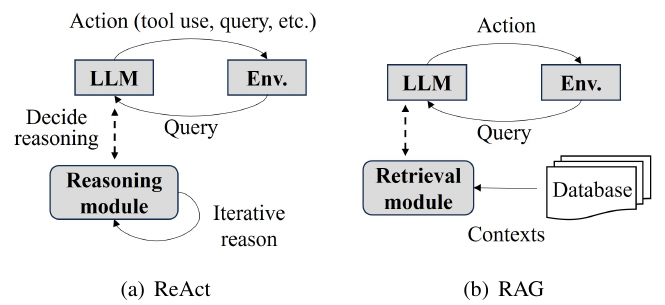
\includegraphics[width=0.85\linewidth]{fig/fig10.png}
\caption{ReAct와 RAG의 개념도.}
\label{fig:10}
\end{figure}

ReAct 원리는 의미 통신으로 확장되었다 [130].
여기서 ASC는 ReAct 메커니즘을 다중 에이전트 계획 프레임워크로 일반화한다.
각 에이전트는 관측을 바탕으로 내부 추론과 외부 실행을 번갈아 수행하며 앞으로의 결정을 반복적으로 다듬는다.
이때 프롬프트 수준의 명시적 추론 흔적은 실제 통신에 필요하지 않으므로 생략한다.
마찬가지로 [129], [131]의 연구는 기존 LLM 기반 방법이 대역폭 할당과 변조 방식을 결합 최적화하지 못함을 보였다.
이 문제를 해결하기 위해, 그림~11에 보인 것처럼 계획 능력을 갖춘 인지 의미 통신 에이전트가 효율적인 자원 할당과 중계기 선택을 가능하게 한다 [129].
더 나아가 과업 계획은 오토인코더 기반 의미 통신이 분포 이동에 민감한 문제를 완화한다 [131].

\setcounter{figure}{10}
\begin{figure}[htbp]
\centering
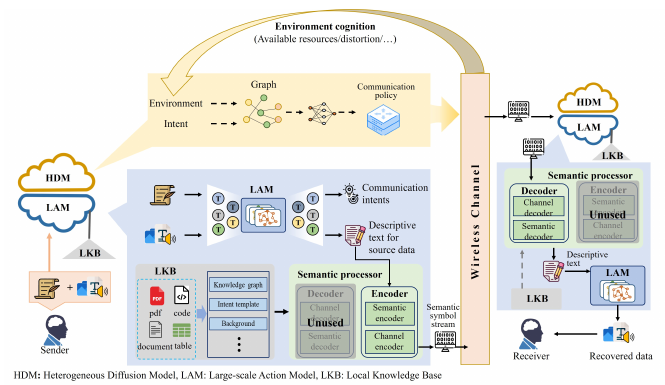
\includegraphics[width=\linewidth]{fig/fig11.png}
\caption{계획 능력을 갖춘 ASC의 프레임워크 예시 [129].}
\label{fig:11}
\end{figure}

RAG는 적응성과 의미적 신뢰성을 높이기 위해 ASC에 적용되었다 [132]--[135].
[132]에서는 검색 증강 다중 모달 의미 통신(RAMSC, retrieval-augmented multimodal SC) 프레임워크를 도입하여, 국소 캐싱과 선택적 검색으로 핵심 다중 모달 요소를 효율적으로 교환할 수 있게 했다.
이를 통해 RAMSC 프레임워크는 정적 검색 방법에 비해 통신 오버헤드를 줄인다.
다른 연구에서는 적용 범위를 넓히기 위해 RAG를 생성형 AI(GAI)와 통합했다 [133].
[133]에 따르면 GAI를 결합한 RAG 방법은 환각 아티팩트를 완화하고 복원 품질을 높인다.
마찬가지로 구조화된 의미 삼중항(semantic triple)과 RAG를 사용하는 개인화 전송 프레임워크 [134]는 의미 콘텐츠 전달의 신뢰성을 한층 강화한다.
통신 시스템에 RAG를 통합함으로써 동적 네트워크의 최적화가 쉬워졌다 [135].
RAG 지식을 활용하면 통신 시스템의 최적화 문제를 자동으로 정식화할 수 있어, 수작업 설계에 비해 모델링 오류가 크게 줄어든다.

RAG는 지식이 보호되는 한 안전한 전송도 보장할 수 있다.
구체적으로, 송신기는 의도한 의미를 나타내는 최소 부분 그래프의 노드 식별자를 전송한다.
수신기는 LLM용으로 생성한 프롬프트를 사용해 자신의 국소 지식 그래프(KG)에서 내용이나 의도를 복원한다 [136].
이 과정은 전송되는 민감 정보의 노출 면을 줄일 수 있다.
그러나 KB에 대한 무단 접근이나 KB의 손상은 정보 유출이라는 새로운 위험을 낳을 수 있으므로, 강건한 정보 보호 전략이 필요하다.
최근 연구 [137]에서는 적대적 학습, 데이터 검증, 이상 탐지 같은 다양한 전략을 사용해 정보 유출이나 조작에 맞서 통신에서 RAG의 보안을 높일 수 있음을 보였다.

LLM을 ReAct나 RAG 방법으로 ASC 프레임워크에 통합하면, 토큰 크기나 처리량과 관련된 통신 오버헤드는 줄지만 추론 지연은 늘어난다.
추론 비용의 균형을 맞추기 위해 ``Plan-and-Act'' [138] 같은 계층적 계획 구조가 등장했다.
이 구조에서 LLM은 상위 수준 계획을 세우는 계획기 역할을 하고, 가벼운 실행기가 그 계획을 효율적으로 실행한다.
``Plan-and-Act'' 개념은 ASC에 Talker--Reasoner 구조로 도입되었다 [37].
이 구조에서 저지연 Talker(시스템 1)는 일반적인 질의를 처리하고, Reasoner(시스템 2)는 불확실성이 높은 상황에서 호출된다.

최근에는 상위 수준의 사용자 의도를 네트워크 구성으로 변환하는 에이전트형 맥락 검색 프레임워크가 제안되었다 [139].
의미 임베딩에 의존하는 RAG 접근과 달리, 이 에이전트형 프레임워크는 다중 출처 지식 검색, CoT 추론, 자기 검증을 통합하여 의사 결정 정확도를 높인다.
그 결과 지능형 기지국은 표준을 준수하는 정책 시행과 관련된 통신 시스템의 복잡한 과업을 자율적으로 수행할 수 있다.

\paragraph{3) 메모리}
ASC 안에서 메모리 모듈은 사용자 행동과 환경 맥락을 비롯해 전송으로부터 얻은 의미 정보를 저장할 수 있다 [140].
또한 최근 연구들은 의미 충실도와 맥락 이해를 높이기 위해 외부 메모리를 도입할 수 있음을 보였다 [117], [141].
구체적으로, 메모리 DeepSC(MeM-DeepSC) [117]는 맥락 정보를 처리하는 메모리 요소를 도입하여, 답변 정확도와 전송 심볼 수 측면에서 기존 의미 통신 모델보다 개선된 결과를 보였다.
메모리를 활용하는 또 다른 방식으로, 확장 맥락 기반 의미 통신은 과거 통신 텍스트라는 개념을 사용한다 [141].
이 의미 통신 프레임워크는 이전에 저장한 문장을 문장 복호 과정에서 추가 맥락으로 재사용하여 정확도를 높였다.

최근 연구들은 맥락 강화보다는 전송 효율을 높이기 위한 메모리 사용을 탐구했다.
진화형 의미 통신 프레임워크 [142]에서는 중복 전송을 피하기 위해 의미 캐싱 전략을 사용한다.
새 의미 벡터가 메모리에 저장된 벡터와 유사하면, 시스템은 일치한 벡터의 인덱스만 전송한다.
또 다른 접근 [143]은 정적 부호책을 갖춘 메모리 기반 분류 모델을 채택한다.
시스템은 가장 가까운 부호책 항목을 선택해 의미 양자화를 수행하고, 해당 인덱스를 전송한다.
이런 방식으로 메모리를 사용하면 학습 오버헤드가 줄고 시간 효율이 높아진다.

\paragraph{4) 자기 교정}
LLM에서 오류를 자율적으로 식별하고 교정하는 능력을 자기 교정(self-correction)이라 한다 [144].
초기 연구는 주로 외부 되먹임 없이 오류를 바로잡는 LLM 고유의 능력에 초점을 맞추었다 [145].
그러나 LLM은 고유 능력만으로는 오류를 교정하는 데 어려움을 겪는다는 사실이 밝혀졌다 [145].
예를 들어 외부 되먹임이 없는 LLM은 올바른 응답을 수정해 버려 성능이 떨어질 수 있다 [146].
이에 따라 후속 연구는 외부 되먹임이나 미세 조정을 통해 자기 교정을 개선하는 데 초점을 맞추었다 [147].
자기 교정 과정에 자기 비판을 통합함으로써 LLM의 정확도가 더욱 향상되었다 [147].

ASC 시스템에서 자기 교정은 에이전트가 자율적으로 개선하는 능력을 가리킨다 [119].
이러한 자기 교정은 에이전트가 자신의 사고 과정을 평가하고 개선하는 능력인 메타인지(meta-cognition)에 해당한다.
의미 오류는 두 유형으로 분류된다.
하나는 가우스 과정 의미 오류이고, 다른 하나는 인간 참여형 강화학습(HITL-RL, human-in-the-loop reinforcement learning) 의미 오류다.
가우스 과정 오류는 잠재 공간에서 이상값으로 식별되며, 데이터 분포 이동, 채널 변동, 적대적 공격 같은 객관적 요인에서 비롯된다 [148].
이와 달리 HITL-RL 오류는 사용자 선호 같은 주관적 변화에서 비롯되며, 인간 되먹임을 활용한 DRL로 바로잡는다 [119].
최근의 발전은 전문가의 도움 없이도 DRL을 통해 자기 교정을 효과적으로 이끌어 내거나 구현할 수 있음을 보여 주었다 [115], [149].
